\section{Prozesse und Threads}

Viele modernen Betriebssysteme können mehrere Operationen gleichzeitig ausführen. Das Ausführen eines Browsers und eines Textverarbeitungsprogramm stellt für moderne Betriebssysteme keine Schwierigkeit mehr dar. Dieses Kapitel gibt einen Überblick über grundlegende Konzepte von concurrency und paralleler Programmierung. Um einen tieferen Einblick in dieses Thema zu erlangen bietet sich das Kapitel 2 aus dem Buch Moderne Betriebssysteme von Andrew S. Tannenbaum an. 

\subsection{Prozess}
\label{section: Prozess}
Tannenbaum beschreibt einen Prozess als ein Programm welches sich in Ausführung befindet. Ein Prozess beinhaltet den aktuellen Wertes des Befehlszählers, die Registerinhalte und die Belegung der Variablen. Um den Anschein von Parallelität zu erwecken wechselt das Betriebssystem zwischen einzelnen Prozessen und kann so mehr Prozesse verarbeiten als die CPU Kerne besitzt. Welcher Prozess wann ausgeführt wird entscheidet ein Scheduling Algorithmus. Dieser koordiniert die einzelnen Prozesse und vergibt Rechenzeit auf der CPU. Dadurch kann ein Betriebssystem, welches auf einem Computer mit Single Core Prozessor arbeitet, den Anschein erwecken als ob mehrere Applikationen parallel laufen würden. Zum Beispiel kann ein Textverarbeitungsprogramm ausgeführt werden und gleichzeitig ein Browser geöffnet sein \cite[p. 87]{tan09}.

\subsection{Threads}
\label{section: Threads}
Ein Prozess besitzt immer nur einen Ausführungsfaden. Mehrere Prozesse können parallel oder quasi-parallel abgearbeitet werden. Es gibt Situationen in denen eine Applikation mehrere Ausführungsfäden parallel bearbeiten möchte und gleichzeitig auf den selben Adressraum zugreifen möchte. Threads bieten die Möglichkeit mehrere Ausführungsfäden in einem Prozess zu behandeln. Das Ausführen von mehreren Threads in einem Prozess wird als Multithreading bezeichnet. Dabei besitzt ein Thread einen Befehlszeiger, ein Register und einen eigenen Stack. Der Befehlszeiger gibt an welcher Befehl als nächstes ausgeführt werden soll. Das Register beinhaltet alle lokalen Variablen. Im Stack werden aufgerufene Funktionen gestapelt, welche noch nicht verlassen wurden. Durch den geteilten Adressraum besitzen alle Threads des Prozesses die selben globalen Variablen. Einzelne Threads können diese globalen Variablen lesen, modifizieren und löschen \cite[p. 97]{tan09}. 

Bei der Realisierung von Threads kann man prinzipiell zwischen drei Arten unterscheiden\footnote{Auf Threads in Kernel und Hybride Realisierungen wird in dieser Arbeit nicht eingegangen. Eine Einführung in Kernel Threads und Hybride Threads findet sich in \cite[p. 109-110]{tan09}}:

\begin{itemize}
  \item Threads im Benutzeradressraum
  \item Threads im Kernel 
  \item Hybride Realisierung von Threads
\end{itemize}

Werden Threads im Benutzerraum implementiert so weiß das Betriebssystem nichts von den einzelnen Threads. Das Erstellen, Löschen und Scheduling dieser Threads muss von der Laufzeitumgebung  behandelt werden. Die Laufzeitumgebung muss dafür eine eigene Thread Tabelle verwalten. Die Implementierung von Threads im Benutzeradressraum wird auch als Green-Threads bezeichnet. Green Threads können schneller sein als Betriebssystem Threads, da sie einen für den Anwendungsfall angepassten Scheduling Algorithmus besitzen können \cite[p. 106-108]{tan09}.

Bei Kernel-Threads werden die Threads direkt vom Kernel des Betriebssystems verwaltet. Um einen neuen Thread zu erstellen oder zerstören muss ein Systemaufruf getätigt werden. Möchte ein Prozess einen Systemaufruf tätigen übergibt der Prozess die Kontrolle an das Betriebssystem. Der Wechsel vom Benutzeradressraum in den Kernel verursacht eine kurze Unterbrechung. Aus diesem Grund zerstörten manche Betriebssysteme Threads nicht wirklich, sondern reaktivieren diese sobald ein neuer Thread erstellt werden soll \cite[p. 59, p. 106-108]{tan09}.


\subsection{Prozesse vs. Threads}

Prozesse und Threads teilen sich einige Eigenschaften. Beide Konzepte bieten die Möglichkeit Aufgaben parallel oder pseudo parallel zu bearbeiten. Prozesse teilen sich physische Ressourcen eines Computers wie Speicher, Festplatten, I/O Geräte, etc. Threads teilen sich den Adressraum und geöffnete Dateien eines Prozesses. Prozesse gehören immer zu genau einem Benutzer eines Betriebssystems. Threads hingegen gehören zu einem Prozess und besitzen dadurch nur indirekt einen Benutzer \cite[p. 89]{tan09}. 


\subsection{Probleme bei Verwendung von Threads}
Bei der Verwendung von mehreren Threads in einer Applikation können durch den geteilten Adressraum einige Probleme auftreten. In vielen Fällen entstehen Probleme bei der Synchronisation der Daten. Race Conditions und Deadlocks sind zwei häufig auftretende Probleme bei der Verwendung Multithreading. 

\subsubsection{Context Switching}
Um einen möglichst fairen Zugriff auf die CPU zu bieten kann das Betriebssystem einzelne Threads zu jeder Zeit stoppen und zu einem späteren Zeitpunkt wieder ausführen. Der Zeitpunkt wann ein Thread gestoppt und wieder ausgeführt werden soll, wird von dem \emph{Scheduling Algorithmus} bestimmt. Die Übergabe von CPU Ressourcen von einem Thread an den anderen wird als Context-Switch bezeichnet. Dabei spielt es keine Rolle ob die Threads im Benutzeradressraum oder im Kernel des Betriebssystems implementiert wurden \cite[p. 23]{Sto2013}.

\subsubsection{Race Conditions}

Eine Race Condition tritt auf wenn mindestens zwei Threads (Thread A und B) auf die selbe Speicheradresse zugreifen und diese vom jeweils anderen Thread unerwarteterweise verändert wird. Eine unerwartete Veränderung kann durch paralleles Ausführen zweier Threads oder durch einen Context-Switch entstehen. Bei einem Context-Switch kann eine Race-Condition auftreten, wenn der Scheduling Algorithmus in einer kritischen Phase von Thread A entscheidet, dass Thread B die CPU Ressourcen zur Verfügung gestellt bekommt. Da beide Threads den gleichen Adressraum besitzen darf Thread B auf die selben Werte wie Thread A zugreifen und diese auch verändern.  Thread B verändert einen Wert, welcher von Thread A aktiv genutzt wird. Nachdem Thread A seine Arbeit wieder aufgenommen hat arbeitet dieser mit einem falschen Wert weiter \cite[p. 89]{tan09}. 

Ein Beispiel einer Race Condition zeigt Listing \ref{listing:race_conditions}. Dabei soll der Wert einer Variable ausgegeben werden, wenn dieser 10 ist.

\begin{lstlisting}[
  caption={Race Condition},
  label=listing:race_conditions
]
if x == 10
  # Ein anderer Thread veraendert die Variable x auf 12
  puts x # Output ist 12 
end
\end{lstlisting}

In Listing \ref{listing:race_conditions} ist zu sehen, dass durch einen anderen Thread die Variable x auf einen anderen Wert gesetzt wird. Dadurch wird ein falscher Wert auf der Konsole ausgegeben. Dieses Verhalten ist in vielen Fällen nur schwer reproduzierbar, da der Scheduling Algorithmus schwer vorhersehbar ist \cite[]{Net92}.

\subsubsection{Deadlocks}

In einem Deadlock befinden sich mehrere Threads, die jeweils auf eine Ressource warten, welche vom jeweilig anderen Thread gesperrt ist \cite[p. 1]{Jah04}. Dadurch kann keiner der Threads einen Fortschritt machen und bleiben in diesem Zustand bis der Prozess von einer außenstehenden Prozedur terminiert wird. Deadlocks sind nicht nur auf Threads beschränkt, sondern können auch vorkommen wenn mehrere Prozesse auf die Freigabe von Geräten, Dateien oder Speicherstellen warten. Ein Deadlock kann auch PC übergreifend über ein Netzwerk entstehen \cite[p. 177]{tan09}. 

\emph{The Dining Philosophers Problem:}

Edsger Dijkstra beschreibt in seiner Thesis \emph{Hierarchical ordering of sequential processes} das Problem des Deadlocks anhand von fünf Philosophen, die gemeinsam an einem Tisch sitzen. Dabei beschreibt er folgendes Problem:

\begin{quote}
  Five philosophers numbered 0 through 4 are living in a house where the table laid for them, each philosopher has his own place at the table. Their only problem - besides those of philosophy - is that the dish served is a very difficult kind of spaghetti, that has to be eaten with two forks. There are two forks next to each plate, so that presents no difficulty: as a consequence, however, no two neighbours may be eating simultaneously. \cite[p. 21]{dij71}
\end{quote} 

\begin{figure}[!htb]
  \centering
  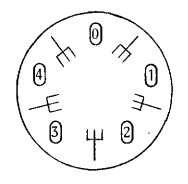
\includegraphics[width=8cm]{images/philosophers.png}
  \caption{
    The Dining Philosophers Problem \cite[p. 21]{dij71} 
  }
  \label{figure:philosophers}
\end{figure}

Alle Philosophen sind mit ihren Gedanken so beschäftigt, dass sie nicht miteinander kommunizieren können. Damit einer der Philosophen essen kann benötigt er beide Gabeln. Eine mögliche Reihenfolge der Operationen die nötig sind damit ein Philosoph essen kann lautet wie folgt \cite[p. 21]{dij71}:

\begin{enumerate}
  \item Denke nach
  \item Ist der Philosoph nicht hungrig? Gehe zu Schritt 1
  \item Ist die rechte Gabel nicht frei, Gehe zu Schritt 1
  \item Nimm die rechte Gabel
  \item Ist die linke Gabel nicht frei, denke nach und wiederhole diesen Schritt
  \item Nimm die linke Gabel
  \item Esse
  \item Lege rechte Gabel auf den Tisch  
  \item Lege linke Gabel auf den Tisch
  \item Gehe zu Schritt 1
\end{enumerate}

Das Problem bei dieser Implementierung ist die Möglichkeit eines Deadlocks. Dieses kann entstehen wenn alle Philosophen zur exakt gleichen Zeit hungrig werden und die jeweils rechte Gabel in die Hand nehmen. Nachdem die jeweils linke Gabel vom rechten Philosophen bereits besetzt ist, denken alle Philosophen so lange nach bis die jeweilige linke Gabel frei wird. Nachdem alle Philosophen die rechte Gabel so lange für sich beanspruchen bis sie nicht mehr hungrig sind wird keiner der Philosophen jemals satt werden \cite[p. 21]{dij71}. 

Das \emph{Dining Philosophers Problem} kann auf die Informatik angewendet werden bei dem mehrere parallel laufende Threads oder Prozesse auf geteilte Ressourcen warten, welche vom jeweilig anderen Thread blockiert wird.

\subsection{Zusammenfassung}
In diesem Kapitel wurden die Grundlagen von Prozessen und Threads näher erläutert. Prozesse können als Programme bezeichnet werden, welche sich in Ausführung befinden. Dabei kann ein Betriebssystem mehrere Programme gleichzeitig ausführen. Dabei besitzen Prozesse einen linearen Programmfluss. Prozesse besitzen einen linearen Programmfluss welcher durch Threads aufgebrochen werden kann.

Durch den nichtlinearen Programmierfluss und das gleichzeitige Behandeln mehrere Prozeduren im selben Adressraum können Race Conditions auftreten. Dabei werden Speicherstellen unerwartet verändert und führen zu korrupten Daten. Deadlocks sind ein weiteres Problem, welche im Zusammenhang von paralleler Programmierung auftreten kann. Diese treten auf, wenn mehrere Prozeduren auf eine Ressource warten, welche vom jeweilig anderen für sich alleine beansprucht wird. Dadurch macht keiner der Prozeduren einen Fortschritt. 